\documentclass[../main.tex]{subfiles}

\begin{document}

%%%%%%%%%%%%%%%%%%%%%%%%%%%%%%%%%%%%%%%%%%%%%%%%%%%%%%%%%%%%%%%%%%%%%%%%%%%%%%%%%%%%%%%%%%%%%%%%%%%%%%%%%
\section{Vázané extrémy}

\begin{theorem}[O hledání extrému funkcí s vazbami]
	Buďte $f,g_1, ... , g_k$ reálné funkce definované na otevřené množině $D \subseteq \mathbb{E}_n$.
	Nechť mají spojité parciální derivace. Nechť je hodnost matice
	\[ M = \begin{pmatrix}
	\frac{\partial g_1}{\partial x_1} & \dots & \frac{\partial g_1}{\partial x_n}\\
	\vdots & \ddots & \vdots\\
	\frac{\partial g_k}{\partial x_1} & \dots & \frac{\partial g_k}{\partial x_n}\\
	\end{pmatrix}\]
	maximální, tedy $k \leq n$, v každém bodě oboru $D$.

	Jestliže funkce $f$ nabývá v bodě $\mathbf{a} = (a_1, ... , a_n)$ lokálního extrému podmíněného vazbami
	\[ \forall i \in \{ 1, ... , k \} \quad g_i(x_1, ... , x_n) = 0\]
	Pak existují čísla $\lambda _1, ... , \lambda _k$ taková, že $\forall i \in {1, ... , n}$ platí
	\[ \frac{\partial f(\mathbf{a})}{\partial x_i} + \sum_{j=1}^{k}\lambda_j \cdot \frac{\partial g_j(\mathbf{a})}{\partial x_i} = 0 \]
	nebo ekvivalentně přes gradienty jako
	\[ \nabla f(\mathbf{a}) + \mbox{\boldmath$\lambda$} \cdot \nabla g(\mathbf{a}) = 0\]
\end{theorem}

\begin{intuition}
	Je-li extrém na hranici vazby, tak parciální derivace funkce v daném bodě budou nějaký násobek parciálních derivací funkce (budou se „dotýkat“) (viz \ref{fig:lag}).
	Koeficientům \(\lambda_i\), který určují tento násobek, se říká \textbf{Lagrangeovy multiplikátory}.

	\begin{figure}[h]
		\centering
		\subfloat[\centering Vázané extrémy v \(\mathbb{R}^2\)]{{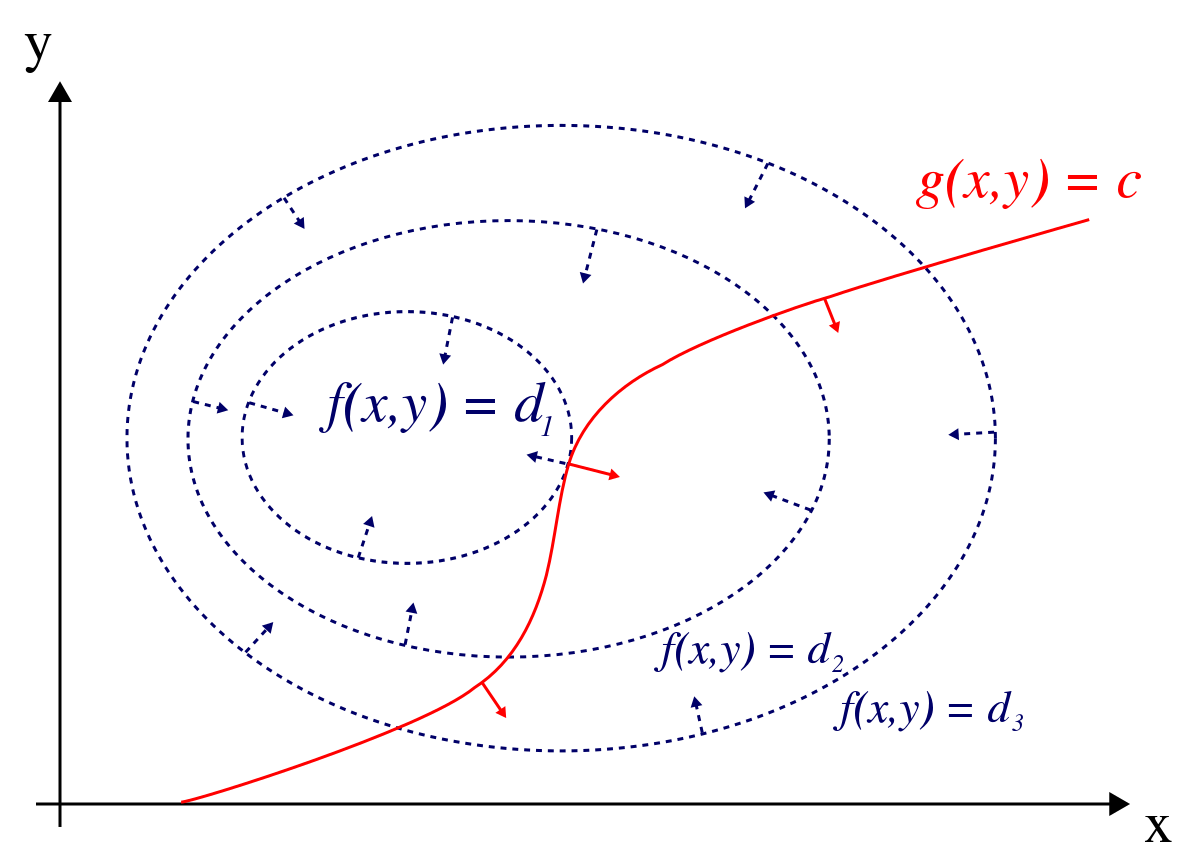
\includegraphics[height=5cm]{05-lagrange-2} }}%
		\hspace{3em}
		\subfloat[\centering Vázané extrémy ve \(\mathbb{R}^3\)]{{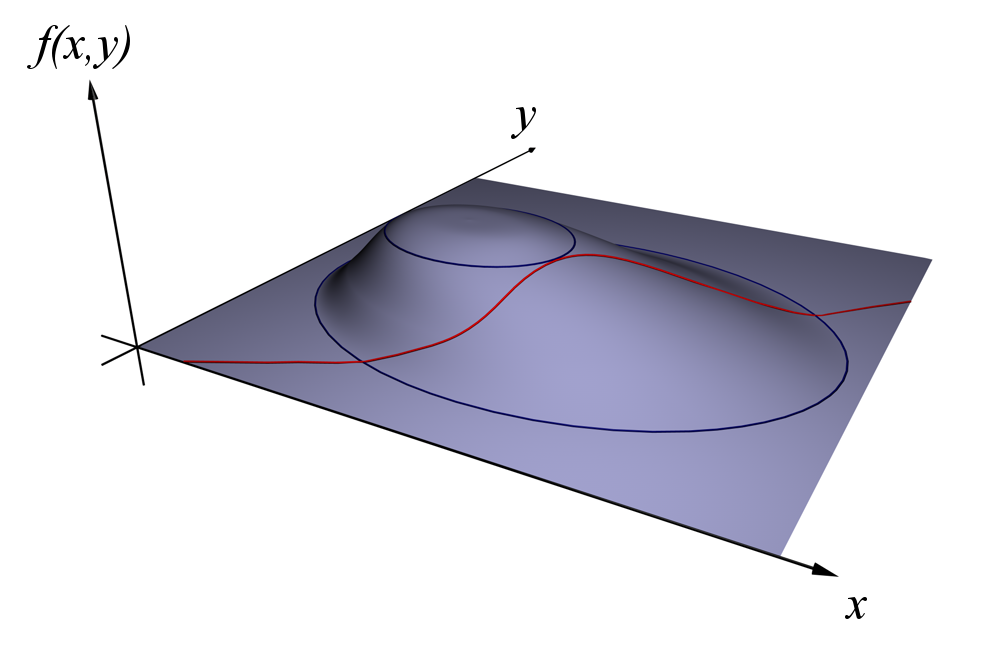
\includegraphics[height=5cm]{05-lagrange-1} }}%
		\caption{Geometrický náhled na počítání vázaných extrémů.}%
		\label{fig:lag}
	\end{figure}
\end{intuition}

\begin{intuition}
	Uvažme funkci \(f(x, y) = 2x + y\) s omezením \(g(x, y) = x^2 + y^2 - 1\).
	Jelikož funkce splňuje předpoklady věty o hledání extrému funkcí, tak můžeme přes Lagrangeovy multiplikátory najít body podezřelé z extrémů.
	Spočítejme je dosazením do definice:
	\[\begin{aligned}
		\frac{\partial f(\mathbf{a})}{\partial x_i} + \sum_{j=1}^{k}\lambda_j \cdot \frac{\partial g_j(\mathbf{a})}{\partial x_i} &= 0 \\
		\frac{\partial f(\mathbf{a})}{\partial x_i} &= \sum_{j=1}^{k}-\lambda_j \cdot \frac{\partial g_j(\mathbf{a})}{\partial x_i} \\
		\begin{bmatrix} \frac{\partial f}{\partial x} \\[6pt] \frac{\partial f}{\partial y} \end{bmatrix} &= -\lambda_1 \begin{bmatrix} \frac{\partial g}{\partial x} \\[6pt]  \frac{\partial g}{\partial y} \end{bmatrix} \\
			\begin{bmatrix} 2 \\ 1 \end{bmatrix} &= -\lambda_1 \begin{bmatrix} 2x \\ 2y \end{bmatrix}
	\end{aligned}\]

	Z toho vyplývá, že hledáme body, které splňují následující rovnice:
	\[\begin{aligned}
		2x \lambda &= -2 \\
		y \lambda &= -1 \\
		g(x, y) = x^2 + y^2 &= 1 \\
	\end{aligned}\]

	Jejich vyřešením (3 rovnice, 3 proměnné) dostáváme dvě řešení \(\left(\frac{2}{\sqrt{5}}, \frac{1}{\sqrt{5}}\right)\) a \(\left(\frac{-2}{\sqrt{5}}, \frac{-1}{\sqrt{5}}\right)\), které jsou minimum a maximum (viz obrázek \ref{fig:lagex}).
		

	\begin{figure}[h]
		\centering
		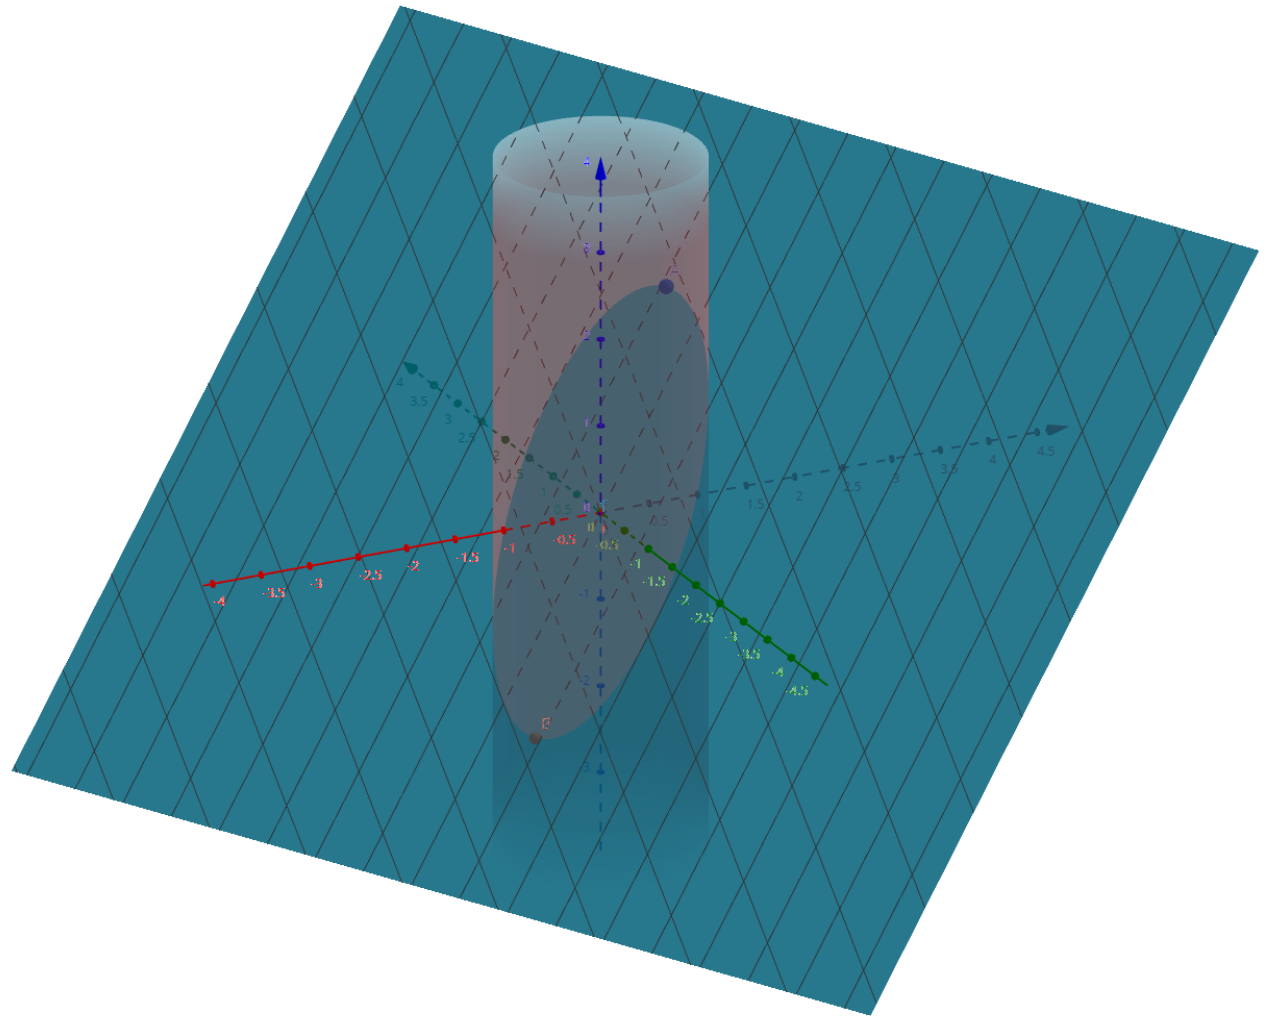
\includegraphics[height=6cm]{05-lag-example}%
		\caption{Geometrický pohled na řešený příklad: \(f\) je modrá, \(g\) červená a extrémy jsou dva viditelné body (maximum modré, minimum červené). Vygenerováno přes GeoGebru [\href{https://www.geogebra.org/3d?lang=en}{odkaz}].}%
		\label{fig:lagex}
	\end{figure}
\end{intuition}

\begin{proof}
	Matice $M$ má hodnost $k$ právě když aspoň jedna její $k\times k$ podmatice $M$ je regulární (a tedy má nenulový determinant). Dejme tomu,
	\[ 0 \neq \begin{vmatrix}
	\frac{\partial g_1}{\partial x_1} & \dots & \frac{\partial g_1}{\partial x_k}\\
	\vdots & \ddots & \vdots\\
	\frac{\partial g_k}{\partial x_1} & \dots & \frac{\partial g_k}{\partial x_k}\\
	\end{vmatrix}\]
	Potom podle věty o implicitních funkcích máme okolí bodu $\textbf{a}$ funkce $\phi_i(x_{k+1},...,x_n)$
	se spojitými parciálními derivacemi takové, že (pišme $\Tilde{\textbf{x}}$ pro $(x_{k+1},...,x_n))$
	\[g_i(\phi_1(\Tilde{\textbf{x}}),...,\phi_k(\Tilde{\textbf{x}}),\Tilde{\textbf{x}}) = 0 \text{ pro } i=1,...,k.\]
	tedy lokální maximum nebo minimum funkce $f(\textbf{x}$) v $\textbf{a}$ podmíněné danými vazbami dává lokální maximum či minimum (nepodmíněné) funkce
	\[F(\Tilde{\textbf{x}}) = f(\phi_1(\Tilde{\textbf{x}}),...,\phi_k(\Tilde{\textbf{x}}),\Tilde{\textbf{x}}),\]
	v $\Tilde{\textbf{a}}$, a tedy je 
	\[\frac{\partial F(\Tilde{\textbf{a}})}{\partial x_i} = 0 \text{ pro } i = k+1,...,n,\]
	to jest, podle řetízkového pravidla
	\[\sum^k_{r=1}\frac{\partial f(\textbf{a})}{\partial x_r}\cdot \frac{\partial \phi_r(\Tilde{\textbf{a}})}{\partial x_i} + \frac{\partial f(\textbf{a})}{\partial x_i} = 0 \text{ pro } i = k+1,...,n.\]
	čili
	\[\frac{\partial f(\textbf{a})}{\partial x_i} = -\sum^k_{r=1}\frac{\partial f(\textbf{a})}{\partial x_r}\cdot \frac{\partial \phi_r(\Tilde{\textbf{a}})}{\partial x_i} \text{ pro } i = k+1,...,n.\]
	Podobně, derivováním konstantní $g_j(\phi_1(\Tilde{\textbf{x}}),...,\phi_k(\Tilde{\textbf{x}}),\Tilde{\textbf{x}}) = 0$ dostaneme pro $j = 1,...,k$
	\[\sum^k_{r=1}\frac{\partial g_j(\textbf{a})}{\partial x_r}\cdot \frac{\partial \phi_r(\Tilde{\textbf{a}})}{\partial x_i} + \frac{\partial g_j(\textbf{a})}{\partial x_i}=0 \text{ pro } i = k+1,...,n.\]
    čili
    \[\frac{\partial g_j(\textbf{a})}{\partial x_i}=-\sum^k_{r=1}\frac{\partial g_j(\textbf{a})}{\partial x_r}\cdot \frac{\partial \phi_r(\Tilde{\textbf{a}})}{\partial x_i} \text{ pro } i = k+1,...,n.\]
	Dále použijeme znovu vlastnost toho, že determinant je nenulový. Vzhledem k hodnosti matice má systém lineárních rovnic
	\[\frac{\partial f(\textbf{a})}{\partial x_i} + \sum^k_{j=1}\lambda_j\cdot\frac{\partial g_j(\textbf{a})}{\partial x_i} = 0, i = 1,...,k\]
	jediné řešení $\lambda_1,...,\lambda_k.$ To jsou rovnosti z tvrzení, ale jen pro $i \leq k$. Musíme ještě dokázat, že to platí i pro $i > k$. 
	\begin{align*}
	\frac{\partial f(\textbf{a})}{\partial x_i} + & \sum^k_{j=1}\lambda_j\cdot\frac{\partial g_j(\textbf{a})}{\partial x_i}=\\
	= & - \sum^k_{r=1} \frac{\partial f(\textbf{a})}{\partial x_r}\cdot\frac{\partial \phi_r(\Tilde{\textbf{a}})}{\partial x_i} -
	\sum^k_{j=1}\lambda_j\cdot\sum^k_{r=1}\frac{\partial g_j(\textbf{a})}{\partial x_r}\cdot\frac{\partial \phi_r(\Tilde{\textbf{a}})}{\partial x_i} =\\
	= & - \sum^k_{r=1}\left(\frac{\partial f(\textbf{a})}{\partial x_r}+\sum^k_{j=1}\lambda_j\cdot\frac{\partial g_j(\textbf{a})}{\partial x_r}\right)\frac{\partial \phi_r(\Tilde{\textbf{a}})}{\partial x_i}=\\
	= & - \sum^k_{r=1}0\cdot\frac{\partial \phi_r(\Tilde{\textbf{a}})}{\partial x_i}=0.
	\end{align*}
\end{proof}

%%%%%%%%%%%%%%%%%%%%%%%%%%%%%%%%%%%%%%%%%%%%%%%%%%%%%%%%%%%%%%%%%%%%%%%%%%%%%%%%%%%%%%%%%%%%%%%%%%%%%%%%%
\subsection{Regulární zobrazení}
\begin{definition}[Regulární zobrazení]
	Buď $U \subseteq \mathbb{E}_n$ otevřená a nechť mají $f_i$ pro $i \in {1, ... , n}$
	spojité parciální derivace. Výsledné zobrazení
	\[ \mathbf{f} = (f_1, ... , f_n): U \to \mathbb{E}_n \]
	je regulární, jestliže
	\[ \forall \mathbf{x} \in U: \frac{D(\mathbf{f})}{D(\mathbf{x})}(\mathbf{x}) \neq 0 \]
\end{definition}

\begin{intuition}
	Regularita je zobecnění pojmu prostého zobrazení pro vícerozměrná zobrazení.
\end{intuition}

\begin{lemma}[Obraz regulární funkce]
	Je-li $\mathbf{f}: U \to \mathbb{E}_n$ regulární, je obraz $\mathbf{f}[V]$ každé otevřené podmnožiny
	$V \subseteq U$ otevřený.
\end{lemma}

\begin{proof}
	Vezměme $f(\textbf{x}^0) = \textbf{y}^0.$ Definujeme $\textbf{F} : V \times \mathbb{E}_n \rightarrow \mathbb{E}_n$ předpisem
	\[F_i(\textbf{x},\textbf{y}) = f_i(\textbf{x}) - y_i.\]
	Potom je $\textbf{F}(\textbf{x}^0,\textbf{y}^0) = \textbf{0}$
	a $\frac{D(\textbf{F})}{D(\textbf{x})} \neq 0$, 
	a tedy můžeme použít větu o IF a dostaneme 
	$\delta > 0$ a $\Delta > 0 : \forall \textbf{y} : ||\textbf{y} - \textbf{y}^0|| < \delta$ $\exists \textbf{x} : ||\textbf{x} - \textbf{x}^0|| < \Delta$ a 
	$F_i(\textbf{x},\textbf{y}) = f_i(\textbf{x}) - y_i = 0$. To znamená, že máme $\textbf{f}(\textbf{x}) = \textbf{y}$ (pozor, $y_i$ jsou zde proměnné, $x_j$ hledané funkce a
	\[\Omega(\textbf{y}^0,\delta) = \{\textbf{y} : ||\textbf{y} - \textbf{y}^0 || < \delta \} \subseteq \textbf{f}[V].\]
\end{proof}

\begin{lemma}[Inverz regulárního zobrazení]
	Buď $\mathbf{f}: U \to \mathbb{E}_n$ regulární zobrazení. Potom $\forall \mathbf{x}^0 \in U \exists$
	otevřené okolí $V$ takové, že restrikce $\mathbf{f}|V$ je bijekce. Navíc, zobrazení
	$\mathbf{g}: f[V] \to \mathbb{E}_n$ inverzní k $\mathbf{f}|V$ je regulární.
\end{lemma}

\begin{proof}
	Znovu použijeme zobrazení $\textbf{F} = (F_1,...,F_n)$, kde $F_i(\textbf{x},\textbf{y}) = f_i(\textbf{x})-y_i$. Pro dost malé 
	$\Delta > 0$ máme právě jedno $\textbf{x} = \textbf{g}(\textbf{y})$ takové, že $\textbf{F}(\mathbf{g}(\textbf{y}),\textbf{y}) = 0$ a $||\textbf{x} - \textbf{x}^0|| < \Delta$.
	Toto $\textbf{g}$ má navíc spojité parciální derivace. Máme
	\[D(id) = D(\textbf{f}\circ\textbf{g}) = D(\textbf{f})\cdot D(\textbf{g}).\]
	Podle řetízkového pravidla (a věty o násobení determinantů) je 
	\[\frac{D(\textbf{f})}{D(\textbf{x})}\cdot\frac{D(\textbf{g})}{D(\textbf{y})} = \det D(\textbf{f})\cdot \det D(\textbf{g}) = 1\]
	a tedy je pro každé $\textbf{y} \in \textbf{f}[V] \colon \frac{D(\textbf{g})}{D(\textbf{y})}(\textbf{y}) \neq 0$.
\end{proof}

\begin{consequence}
	Prosté regulární zobrazení $\mathbf{f}: U \to \mathbb{E}_n$ má regulární inverzi
	$\mathbf{g}: \mathbf{f}[U] \to \mathbb{E}_n$
\end{consequence}

\end{document}
